\section{Implementierung}
Um das ober

\subsection{Versuchsfahrzeug}
Bevor mit Implementierung des in Kapitel~\ref{Kapitel:Theoretische Grundlagen} entwickelten Umfeldmodells begonnen wird, werden die relevanten Informationen �ber das Versuchsfahrzeug mitsamt die darin eingebauten Sensoren dokumentiert und in der eigentlichen Implementierung parametriert.
\subsubsection{Dimension �ber Versuchsfahrzeug}
Bei Implementierung im Rahmen dieser Arbeit ist es auch bedeutungsvoll, die Position bzw. den belegten Raum des Versuchsfahrzeugs zu modellieren und dokumentieren, was einen konkreten Beitrag zur kollisionsfrei Navigation leistet. Au�erdem ist die Information �ber die Anordnung der Lasersensoren eng verbunden mit der Abmessung des Fahrzeugs. Daher wird die Dimension des Fahrzeugs als ein wichtiges Element betrachtet. Die Abbildung~\ref{fig:DimensionVonAuto} zeigt, dass die wichtige Gr��en von Abmessung des Fahrzeugs parametriert werden. Obwohl die Zeichnungsbema�ung eigentlich redundant ist, wird sie mit Absicht angewendet, um die Darstellung der wichtigen Gr��en sichtbar zu machen. Der Rot Punkt bezeichnet hierbei die Koordinatenursprung des Fahrzeugkoordinatensystem und befindet sich mittig auf der Hinterachse~\citep{Hegerhorst.2018}. Die X-Achse des Fahrzeugkoordinatensystem zeigt die L�ngsrichtung des Fahrzeugs nach vorne~\citep{Hegerhorst.2018}. Die Y-Achse verl�uft senkrecht zur X-Achse und zeigt nach links des Fahrtrichtung. Die Koordinatenursprung dient als ein Bezugspunkt und die Gr��en, z.B. die Lage eines Sensors sowie die Position eines detektierten Objekts, werden nur relativ zu dem Bezugssystem bzw. Fahrzeugkoordinatensystem angegeben. 
\begin{figure}[htbp]
	\centering
	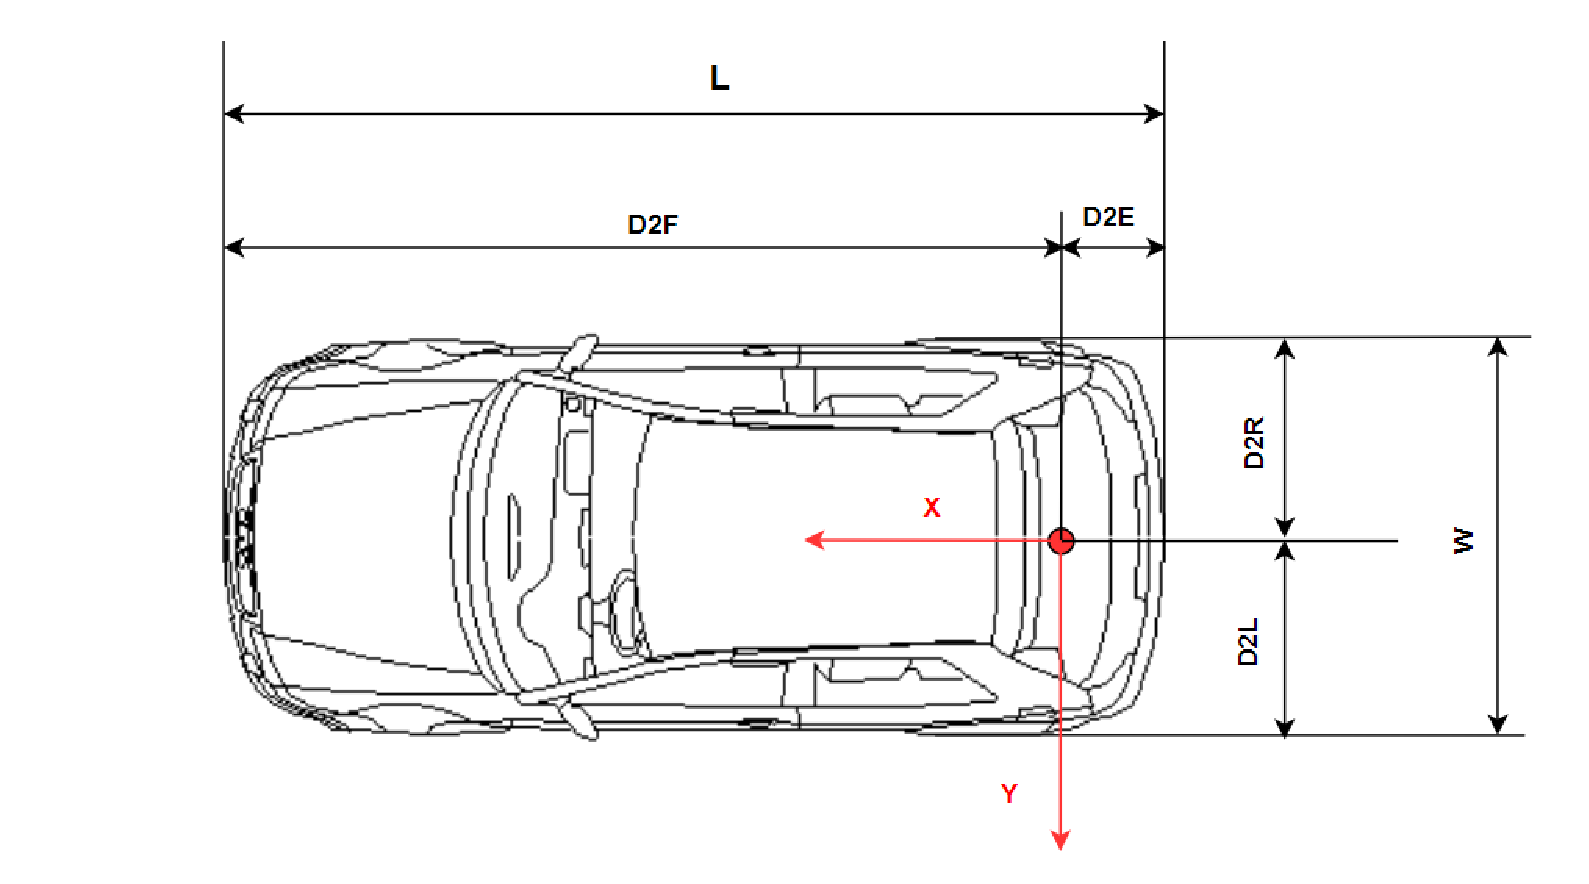
\includegraphics[width=1.0\textwidth]{pics/DimensionVonAuto.pdf}
	\caption{Dimension von Versuchsfahrzeug}
	\label{fig:DimensionVonAuto}
\end{figure}
\\In ifF stehen Golf7 (TIAMO) und Passat Alltrack (TEASY 3) als Versuchsfahrzeuge zur Verf�gung\citep{Hegerhorst.2018}. Die der Abbildung~\ref{fig:DimensionVonAuto} entsprechenden Abmessungen von diesen Versuchsfahrzeugen werden in Tabelle~\ref{tab:Abmessung von Versuchsfahrzeuge} aufgelistet.
\begin{table}[ht]
	\caption{Abmessung von Versuchsfahrzeuge}
	\label{tab:Abmessung von Versuchsfahrzeuge}
	\centering
	\begin{tabular}{|c|c|c|}
		\hline
		\textbf{Abmessung} & \textbf{Golf 7 (TIAMO)} & \textbf{Passat (TEASY 3)}\\
		\hline
		L & $4.3$ & $4.6$\\
		\hline
		W & $1.8$ & $1.6$\\
		\hline
		D2F & $3.5$ & $3.6$\\
		\hline
		D2E & $0.8$ & $1.0$\\
		\hline
		D2L & $0.9$ & $0.8$\\
		\hline
		D2R & $0.9$ & $0.8$\\
		\hline
	\end{tabular}
\end{table}
\subsubsection{Einbauposition der Ibeo-Laserscanner}
Die Anzahl und die Anordnung der im Versuchsfahrzeug installierten Ibeo-Laserscanner dienen auch als wichtigen Parametern bei Implementierung, denn diese Informationen liefern den Startpunkt des Strahls jedes Sensors. In Abbildung~\ref{fig:DimensionVonAuto} sind die Einbauposition und der Erfassungsbereich jedes Sensors dargestellt. Dazu werden die tats�chlichen Werte in Tabelle~\ref{tab:Werte der Einbauposition und des Winkels des Anfangsstrahls jedes Sensors bei TIAMO} und Tabelle~\ref{tab:Werte der Einbauposition und des Winkels des Anfangsstrahls jedes Sensors bei Passat} gegeben. In den Tabellen bezeichnet x die x-Koordinate im Fahrzeugkoordinatensystem und b die y-Koordinate. Der Winkel $\theta$ beschreibt die ausgesandte Richtung des Anfangsstrahls. Der Anfangsstrahl jedes Laserscanners ist gegen den Uhrzeigersinn zur Endstrahl. Der Winkelbereich des Erfassungsraum des Sensors ist nach der Tabelle~\ref{tab:technische Details von Ibeo LUX 8L} auf $110^\circ$ begrenzt. Dieser Wert wird in der Praxis entsprechend der Performance des Umfeldmodells angepasst.
\begin{figure}[htbp]
	\centering
	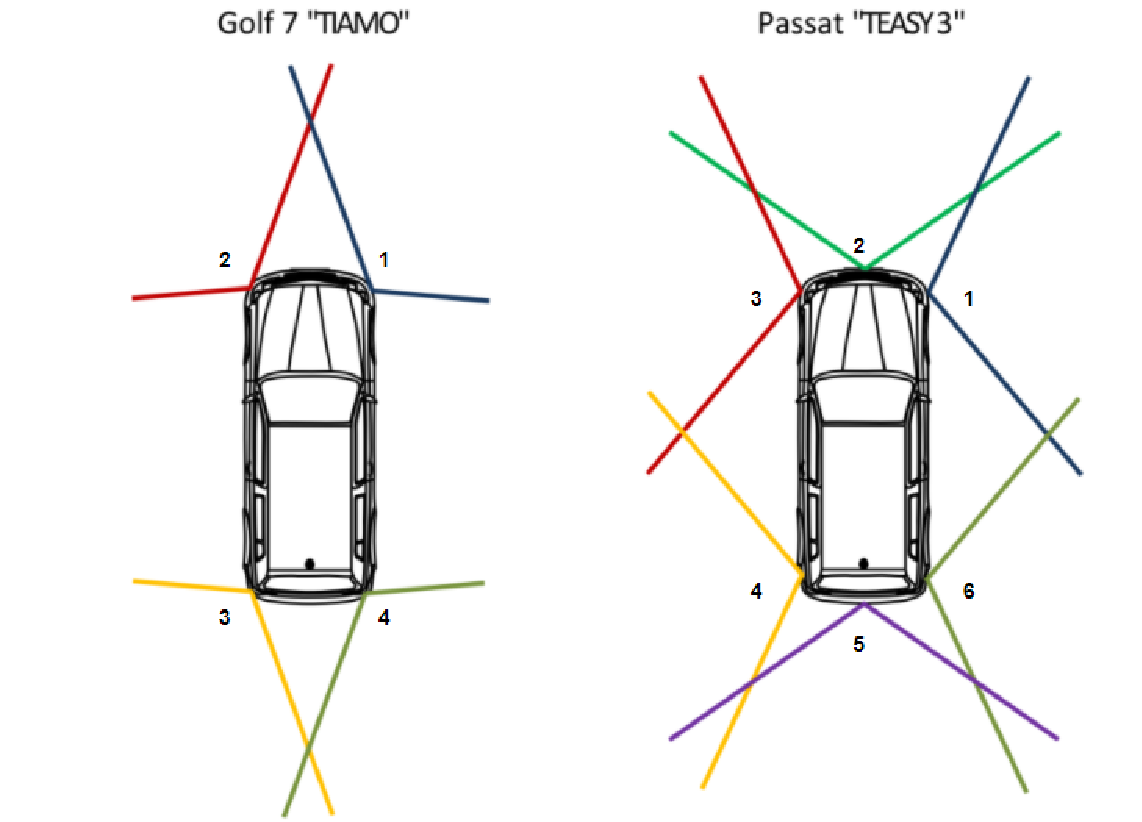
\includegraphics[width=0.7\textwidth]{pics/AnordnungDerLaserscanner.pdf}
	\caption{Einbauposition und Erfassungsbereich der Ibeo-Laserscanner}
	\label{fig:AnordnungDerLaserscanner}
\end{figure}
\begin{table}[ht]
	\caption{Werte der Einbauposition und des Winkels des Anfangsstrahls jedes Sensors bei Golf 7 (TIAMO))}
	\label{tab:Werte der Einbauposition und des Winkels des Anfangsstrahls jedes Sensors bei TIAMO}
	\centering
	\begin{tabular}{|c|c|c|c|}
		\hline
		\textbf{Sensor ID} & \textbf{x (m)} & \textbf{y (m)} & \textbf{Winkel $\theta$ des Anfangsstrahls ($^\circ$)}\\
		\hline
		1 & $3$ & $-0.9$ & $-10$\\
		\hline
		2 & $3$ & $0.9$ & $80$\\
		\hline
		3 & $-0.7$ & $0.9$ & $170$\\
		\hline
		4 & $-0.7$ & $-0.9$ & $-100$\\
		\hline
	\end{tabular}
\end{table}
\begin{table}[ht]
	\caption{Werte der Einbauposition und des Winkels des Anfangsstrahls jedes Sensors bei Passat (TEASY 3)}
	\label{tab:Werte der Einbauposition und des Winkels des Anfangsstrahls jedes Sensors bei Passat}
	\centering
	\begin{tabular}{|c|c|c|c|}
		\hline
		\textbf{Sensor ID} & \textbf{x (m)} & \textbf{y (m)} & \textbf{Winkel $\theta$ des Anfangsstrahls ($^\circ$)}\\
		\hline
		1 & $3.3$ & $-0.8$ & $-35$\\
		\hline
		2 & $3.6$ & $0$ & $45$\\
		\hline
		3 & $3.3$ & $0.8$ & $125$\\
		\hline
		4 & $-0.5$ & $0.8$ & $145$\\
		\hline
		5 & $-1$ & $0$ & $-135$\\
		\hline
		6 & $-0.5$ & $-0.8$ & $-55$\\
		\hline
	\end{tabular}
\end{table}
\subsection{Framework ROS zur Implementierung}
Eine der zentralen Aufgaben dieser Arbeit handelt sich um die Konvertierung von dem am IfF bereits bestehenden MATLAB/Simulink-Modell nach Robot Operating System (ROS).Das Robot Operating System (ROS) ist ein Framework zum Schreiben von Robotersoftware. Es handelt sich um eine Sammlung von Tools, Bibliotheken und Konventionen, die darauf abzielen, die Erstellung komplexer und robuster Roboterverhalten auf einer Vielzahl von Roboterplattformen zu vereinfachen\citep{Quigley.2015}. Obwohl diese Idee aus dem Bereich der Robotik stammt, machen ihre verschiedenen guten Eigenschaften ihre Investition in den Bereich des autonomen Fahrens sehr bedeutsam. Um eine klare Programmstruktur und eine genaue und effiziente Umsetzung des in Kapitel~\ref{Kapitel:Theoretische Grundlagen} genannten Umfeldsmodells zu erhalten, ist eine kurze Einf�hrung in die ROS-Grundlagen und Funktionsmodule in Bezug auf diesen Artikel erforderlich.
\subsubsection{Grundlagen der ROS-Architektur}
Die ROS-Architektur, die in Abbildung~\ref{fig:ROS-Architektur} dargestellt, wurde entworfen und in drei Abschnitte oder Konzeptebenen unterteilt, welche sich um die Dateisystemebene (engl. The Filesystem level), die Berechnungsdiagrammebene (engl. The Computation Graph level) und die Community-Ebene (engl. The Community level) handeln~\citep{Fernandez.2015}.
\begin{figure}[htbp]
	\centering
	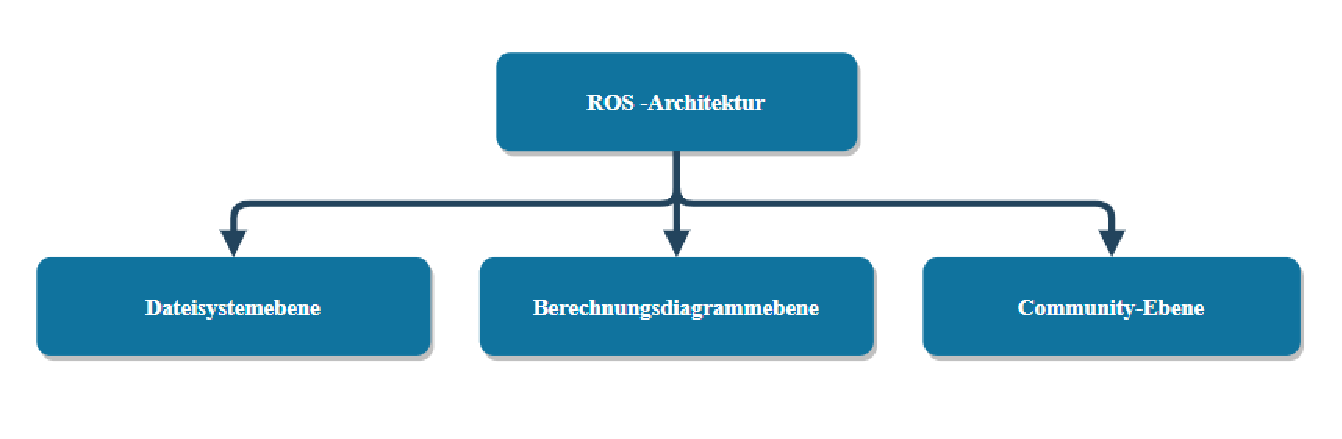
\includegraphics[width=1.0\textwidth]{pics/ROS-Architektur.pdf}
	\caption{ROS-Architektur}
	\label{fig:ROS-Architektur}
\end{figure}
\\Auf der Dateisystemebene wird eine Gruppe von Konzepten verwendet, um zu erkl�ren, wie ROS intern gebildet wird. �hnlich wie bei einem Betriebssystem ist ein ROS-Programm in Ordner unterteilt, und diese Ordner enthalten Dateien, die ihre Funktionen beschreiben~\citep{Fernandez.2015}. Hierbei sind die wichtigen Konzepte zu diesem Artikel Package und Metapackage. Das Package ist die zentrale und grundlegende Dateiorganisationseinheit, die Programmierfunktionen in ROS vollst�ndig realisieren kann. Es enth�lt im Allgemeinen ROS Laufzeitprozess (engl. runtime process), Quellcode (engl. Sourcecode), Konfigurationsdateien (engl. configuration files) und das Package-manifest, das zur Bereitstellung von Informationen von build-dependencies, run-dependencies und Lizenz verwendet wird. Metapackages werden in der Regel nach einer �hnlichen Funktionalit�t gruppiert. Andere Grundkonzepte und Begriffe auf dieser Ebene sind aufgrund der L�nge des Artikels nicht detailliert und finden sich in~\citep{Fernandez.2015}\citep{Koubaa.2016}.
\\Die Berechnungsdiagrammebene ist die relevanteste Ebene f�r diese Arbeit, auf der die Kommunikation zwischen Prozessen und Systemen stattfindet. Die Grundkonzepte auf dieser Ebene sind, wie in Abbildung~\ref{fig:Berechnungsdiagrammebene} dargestellt, Nodes, ROS-Master, Parameter Server, Messages, Topics, Services und ROS-Bags, die alle Daten auf unterschiedliche Weise f�r das Diagramm bereitstellen~\citep{Fernandez.2015}.
\begin{figure}[htbp]
	\centering
	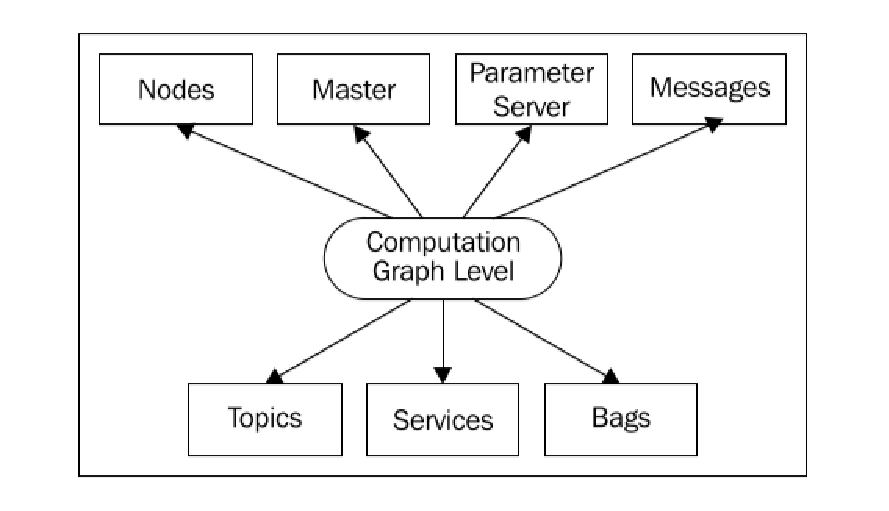
\includegraphics[width=0.7\textwidth]{pics/Berechnungsdiagrammebene.pdf}
	\caption{Wesentliche Grundkonzepte von Berechnungsdiagrammebene}
	\label{fig:Berechnungsdiagrammebene}
\end{figure}
Nodes sind ausf�hrbare Dateien (engl. executables) in ROS und vervollst�ndigen die erwartete Funktion und die zugeh�rigen Berechnungen. Die Nodes k�nnen miteinander kommunizieren und Daten �bertragen. Daher gibt es im Allgemeinen mehrere Nodes in einem System, die unterschiedliche Funktionen ausgef�hrt haben. Der Datenaustausch zwischen Nodes erfolgt �ber Messages. ROS verwendet eine vereinfachte Nachrichtenbeschreibungssprache, um die Datenwerte zu beschreiben, die von Nodes publiziert (engl. published)~\citep{Fernandez.2015}. Damit kann ROS den richtigen Quellcode f�r diese Nachrichtentypen in mehreren Programmiersprachen (z.B. C++ oder Python) generieren. Zahlreiche vordefinierte Messages in ROS k�nnen direkt zum �bertragen von Daten oder zum Erstellen neuer aufgabenorientierter Messages verwendet werden. Dies erfolgt durch Definieren einer Datei mit .msg-Extension. Wenn ein Node Daten sendet, hei�t es, dass das Note eine Topic publizieren. Ein anderer Knoten kann die Topic abonnieren (engl. subscribe), um die Daten abzurufen. Ein Node kann eine Topic nur abonnieren, wenn es denselben Message-Typ hat. Eine Topic kann verschiedene Subsribers und auch verschiedene Publishers haben. Wenn die Kommunikation zwischen Nodes empfangen und beantwortet (engl. receive and reply) werden muss, sollten Services anstelle von Topics verwendet werden. Services geben den Entwicklern die M�glichkeit, mit Nodes zu interagieren. Mit Parameter Server ist es m�glich, Schl�ssel zu verwenden, um Daten an einem zentralen Ort zu speichern und Nodes w�hrend der Ausf�hrung zu konfigurieren oder die Nodes der Knoten zu �ndern~\citep{Fernandez.2015}. Die oben genannte Kommunikation garantiert ROS-Master, der jede Nodes verwalten. Nodes werden zuerst beim Master registriert, und dann integriert der Master Nodes in das gesamte ROS-Programm. Auf diesem Grund besteht der erste Schritt darin, den Master zu starten, wenn das ROS-Programm gestartet wird. ROS-Bag ist ein Format zum Speichern und Wiedergeben aller Informationen der Messages, Topics und Services, die gew�nscht werden. In dieser Arbeit wird ROS-Bag verwendet, um die Sensordaten von dem Versuchsfahrzeug zu speichern. Wenn das ROS-Bag wiedergegeben ist, simuliert es die Datenwerte von Sensoren zu messen und erfassen, was ist praktisch zum Debuggen von Implementierungsalgorithmus.
\\Die Konzepte auf ROS-Community-Ebene sind die ROS-Ressourcen, die es separaten Communities erm�glichen, Software und Wissen auszutauschen~\citep{Fernandez.2015}. Zu den Ressourcen geh�ren unter anderem ROS-Repositories,ROS-Distributions und ROS-Wiki. Jedoch hat diese Ebene f�r diesen Artikel nur eine sehr geringe Relevanz. Auf diesem Grund ist die Auseinandersetzung damit im Rahmen dieser Arbeit zu verzichten.
\\Aufgrund des oben erw�hnten Mechanismus und der Philosophie von ROS hat der Aufbau der Implementierung des Umfeldsmodell auf ROS einen starken Vorteil. Die dezentrale Kommunikationsmethode macht das Implementierungssystem klarer und einfacher. Au�erdem sind Fehler im System leichter zu finden und sortieren. Die Aufteilung zwischen verschiedenen Funktionen erleichtert die sp�tere Systemerweiterung, z.B. Navigation bzw. kollisionsfreie Pfadplanung. Im Rahmen dieser Arbeit ist f�r die Implementierung ROS-Kinetic-Kame mit Ubuntu 16.04 (Xenial) in Benutzung.
\subsubsection{Visualisierung des Umfeldmodells in ROS}